% Created by tikzDevice version 0.12.6 on 2026-07-04 06:01:29
% !TEX encoding = UTF-8 Unicode
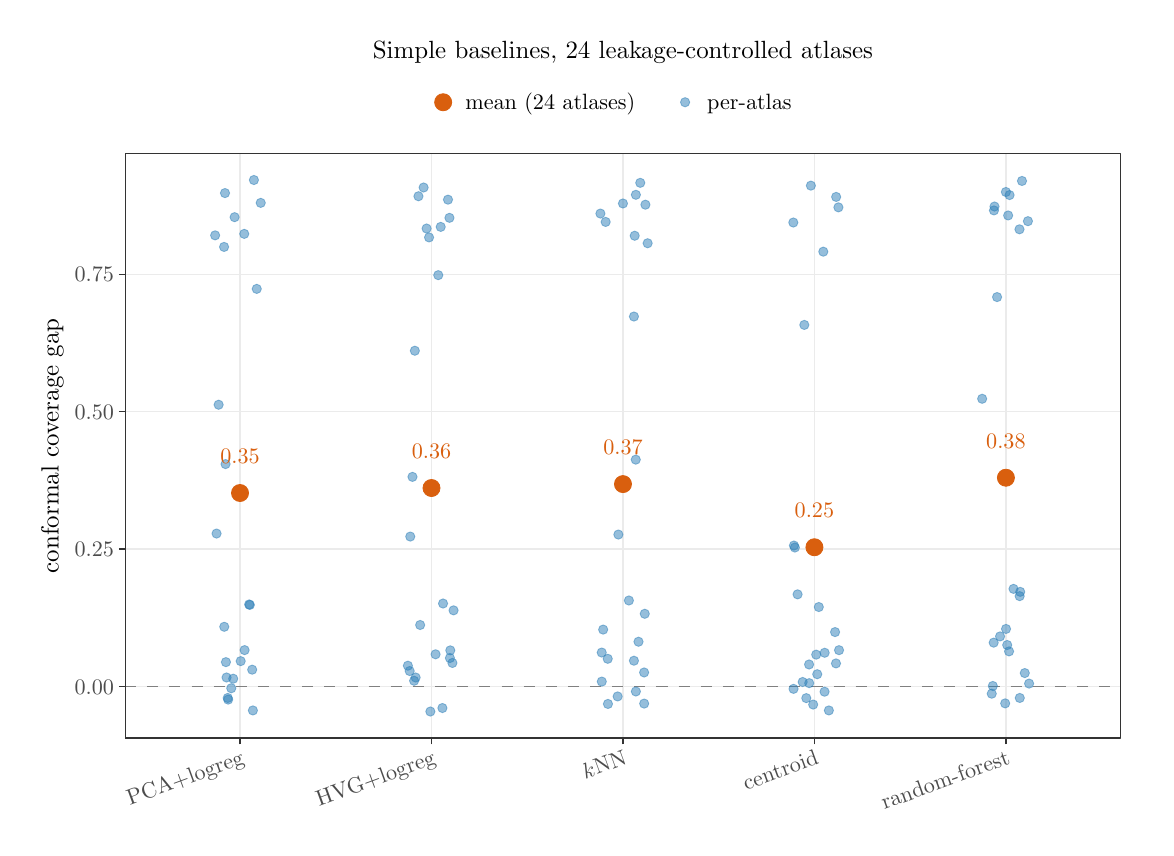
\begin{tikzpicture}[x=1pt,y=1pt]
\definecolor{fillColor}{RGB}{255,255,255}
\path[use as bounding box,fill=fillColor,fill opacity=0.00] (0,0) rectangle (403.99,289.08);
\begin{scope}
\path[clip] (  0.00,  0.00) rectangle (403.99,289.08);
\definecolor{drawColor}{RGB}{255,255,255}
\definecolor{fillColor}{RGB}{255,255,255}

\path[draw=drawColor,line width= 0.5pt,line join=round,line cap=round,fill=fillColor] ( -0.00, -0.00) rectangle (403.99,289.08);
\end{scope}
\begin{scope}
\path[clip] ( 35.22, 32.37) rectangle (394.99,243.63);
\definecolor{fillColor}{RGB}{255,255,255}

\path[fill=fillColor] ( 35.22, 32.37) rectangle (394.99,243.63);
\definecolor{drawColor}{gray}{0.92}

\path[draw=drawColor,line width= 0.5pt,line join=round] ( 35.22, 50.99) --
	(394.99, 50.99);

\path[draw=drawColor,line width= 0.5pt,line join=round] ( 35.22,100.65) --
	(394.99,100.65);

\path[draw=drawColor,line width= 0.5pt,line join=round] ( 35.22,150.30) --
	(394.99,150.30);

\path[draw=drawColor,line width= 0.5pt,line join=round] ( 35.22,199.95) --
	(394.99,199.95);

\path[draw=drawColor,line width= 0.5pt,line join=round] ( 76.73, 32.37) --
	( 76.73,243.63);

\path[draw=drawColor,line width= 0.5pt,line join=round] (145.92, 32.37) --
	(145.92,243.63);

\path[draw=drawColor,line width= 0.5pt,line join=round] (215.11, 32.37) --
	(215.11,243.63);

\path[draw=drawColor,line width= 0.5pt,line join=round] (284.29, 32.37) --
	(284.29,243.63);

\path[draw=drawColor,line width= 0.5pt,line join=round] (353.48, 32.37) --
	(353.48,243.63);
\definecolor{drawColor}{gray}{0.50}

\path[draw=drawColor,line width= 0.5pt,dash pattern=on 4pt off 4pt ,line join=round] ( 35.22, 50.99) -- (394.99, 50.99);
\definecolor{drawColor}{RGB}{44,127,184}
\definecolor{fillColor}{RGB}{44,127,184}

\path[draw=drawColor,draw opacity=0.50,line width= 0.3pt,line join=round,line cap=round,fill=fillColor,fill opacity=0.50] ( 74.77,220.60) circle (  1.68);

\path[draw=drawColor,draw opacity=0.50,line width= 0.3pt,line join=round,line cap=round,fill=fillColor,fill opacity=0.50] (152.41,220.36) circle (  1.68);

\path[draw=drawColor,draw opacity=0.50,line width= 0.3pt,line join=round,line cap=round,fill=fillColor,fill opacity=0.50] (206.96,221.91) circle (  1.68);

\path[draw=drawColor,draw opacity=0.50,line width= 0.3pt,line join=round,line cap=round,fill=fillColor,fill opacity=0.50] (287.50,208.14) circle (  1.68);

\path[draw=drawColor,draw opacity=0.50,line width= 0.3pt,line join=round,line cap=round,fill=fillColor,fill opacity=0.50] (349.16,223.04) circle (  1.68);

\path[draw=drawColor,draw opacity=0.50,line width= 0.3pt,line join=round,line cap=round,fill=fillColor,fill opacity=0.50] ( 67.74,214.03) circle (  1.68);

\path[draw=drawColor,draw opacity=0.50,line width= 0.3pt,line join=round,line cap=round,fill=fillColor,fill opacity=0.50] (149.25,217.09) circle (  1.68);

\path[draw=drawColor,draw opacity=0.50,line width= 0.3pt,line join=round,line cap=round,fill=fillColor,fill opacity=0.50] (208.85,218.88) circle (  1.68);

\path[draw=drawColor,draw opacity=0.50,line width= 0.3pt,line join=round,line cap=round,fill=fillColor,fill opacity=0.50] (276.66,218.67) circle (  1.68);

\path[draw=drawColor,draw opacity=0.50,line width= 0.3pt,line join=round,line cap=round,fill=fillColor,fill opacity=0.50] (358.39,216.22) circle (  1.68);

\path[draw=drawColor,draw opacity=0.50,line width= 0.3pt,line join=round,line cap=round,fill=fillColor,fill opacity=0.50] ( 69.00,152.83) circle (  1.68);

\path[draw=drawColor,draw opacity=0.50,line width= 0.3pt,line join=round,line cap=round,fill=fillColor,fill opacity=0.50] (139.90,172.34) circle (  1.68);

\path[draw=drawColor,draw opacity=0.50,line width= 0.3pt,line join=round,line cap=round,fill=fillColor,fill opacity=0.50] (219.07,184.70) circle (  1.68);

\path[draw=drawColor,draw opacity=0.50,line width= 0.3pt,line join=round,line cap=round,fill=fillColor,fill opacity=0.50] (293.18, 64.14) circle (  1.68);

\path[draw=drawColor,draw opacity=0.50,line width= 0.3pt,line join=round,line cap=round,fill=fillColor,fill opacity=0.50] (350.29,191.73) circle (  1.68);

\path[draw=drawColor,draw opacity=0.50,line width= 0.3pt,line join=round,line cap=round,fill=fillColor,fill opacity=0.50] ( 72.45, 46.28) circle (  1.68);

\path[draw=drawColor,draw opacity=0.50,line width= 0.3pt,line join=round,line cap=round,fill=fillColor,fill opacity=0.50] (149.87, 43.23) circle (  1.68);

\path[draw=drawColor,draw opacity=0.50,line width= 0.3pt,line join=round,line cap=round,fill=fillColor,fill opacity=0.50] (213.18, 47.42) circle (  1.68);

\path[draw=drawColor,draw opacity=0.50,line width= 0.3pt,line join=round,line cap=round,fill=fillColor,fill opacity=0.50] (289.51, 42.36) circle (  1.68);

\path[draw=drawColor,draw opacity=0.50,line width= 0.3pt,line join=round,line cap=round,fill=fillColor,fill opacity=0.50] (358.49, 46.87) circle (  1.68);

\path[draw=drawColor,draw opacity=0.50,line width= 0.3pt,line join=round,line cap=round,fill=fillColor,fill opacity=0.50] ( 74.27, 53.83) circle (  1.68);

\path[draw=drawColor,draw opacity=0.50,line width= 0.3pt,line join=round,line cap=round,fill=fillColor,fill opacity=0.50] (137.39, 58.53) circle (  1.68);

\path[draw=drawColor,draw opacity=0.50,line width= 0.3pt,line join=round,line cap=round,fill=fillColor,fill opacity=0.50] (207.43, 63.28) circle (  1.68);

\path[draw=drawColor,draw opacity=0.50,line width= 0.3pt,line join=round,line cap=round,fill=fillColor,fill opacity=0.50] (282.36, 58.97) circle (  1.68);

\path[draw=drawColor,draw opacity=0.50,line width= 0.3pt,line join=round,line cap=round,fill=fillColor,fill opacity=0.50] (353.52, 71.81) circle (  1.68);

\path[draw=drawColor,draw opacity=0.50,line width= 0.3pt,line join=round,line cap=round,fill=fillColor,fill opacity=0.50] ( 71.30,229.31) circle (  1.68);

\path[draw=drawColor,draw opacity=0.50,line width= 0.3pt,line join=round,line cap=round,fill=fillColor,fill opacity=0.50] (141.21,228.16) circle (  1.68);

\path[draw=drawColor,draw opacity=0.50,line width= 0.3pt,line join=round,line cap=round,fill=fillColor,fill opacity=0.50] (219.77,228.69) circle (  1.68);

\path[draw=drawColor,draw opacity=0.50,line width= 0.3pt,line join=round,line cap=round,fill=fillColor,fill opacity=0.50] (292.96,224.15) circle (  1.68);

\path[draw=drawColor,draw opacity=0.50,line width= 0.3pt,line join=round,line cap=round,fill=fillColor,fill opacity=0.50] (353.48,229.70) circle (  1.68);

\path[draw=drawColor,draw opacity=0.50,line width= 0.3pt,line join=round,line cap=round,fill=fillColor,fill opacity=0.50] ( 71.50,131.38) circle (  1.68);

\path[draw=drawColor,draw opacity=0.50,line width= 0.3pt,line join=round,line cap=round,fill=fillColor,fill opacity=0.50] (139.05,126.76) circle (  1.68);

\path[draw=drawColor,draw opacity=0.50,line width= 0.3pt,line join=round,line cap=round,fill=fillColor,fill opacity=0.50] (219.73,132.99) circle (  1.68);

\path[draw=drawColor,draw opacity=0.50,line width= 0.3pt,line join=round,line cap=round,fill=fillColor,fill opacity=0.50] (277.23,101.23) circle (  1.68);

\path[draw=drawColor,draw opacity=0.50,line width= 0.3pt,line join=round,line cap=round,fill=fillColor,fill opacity=0.50] (344.90,154.98) circle (  1.68);

\path[draw=drawColor,draw opacity=0.50,line width= 0.3pt,line join=round,line cap=round,fill=fillColor,fill opacity=0.50] ( 84.21,225.77) circle (  1.68);

\path[draw=drawColor,draw opacity=0.50,line width= 0.3pt,line join=round,line cap=round,fill=fillColor,fill opacity=0.50] (151.88,226.93) circle (  1.68);

\path[draw=drawColor,draw opacity=0.50,line width= 0.3pt,line join=round,line cap=round,fill=fillColor,fill opacity=0.50] (223.22,225.11) circle (  1.68);

\path[draw=drawColor,draw opacity=0.50,line width= 0.3pt,line join=round,line cap=round,fill=fillColor,fill opacity=0.50] (292.14,227.92) circle (  1.68);

\path[draw=drawColor,draw opacity=0.50,line width= 0.3pt,line join=round,line cap=round,fill=fillColor,fill opacity=0.50] (349.36,224.45) circle (  1.68);

\path[draw=drawColor,draw opacity=0.50,line width= 0.3pt,line join=round,line cap=round,fill=fillColor,fill opacity=0.50] ( 71.86, 54.27) circle (  1.68);

\path[draw=drawColor,draw opacity=0.50,line width= 0.3pt,line join=round,line cap=round,fill=fillColor,fill opacity=0.50] (138.25,105.19) circle (  1.68);

\path[draw=drawColor,draw opacity=0.50,line width= 0.3pt,line join=round,line cap=round,fill=fillColor,fill opacity=0.50] (213.45,105.92) circle (  1.68);

\path[draw=drawColor,draw opacity=0.50,line width= 0.3pt,line join=round,line cap=round,fill=fillColor,fill opacity=0.50] (278.20, 84.31) circle (  1.68);

\path[draw=drawColor,draw opacity=0.50,line width= 0.3pt,line join=round,line cap=round,fill=fillColor,fill opacity=0.50] (358.65, 85.22) circle (  1.68);

\path[draw=drawColor,draw opacity=0.50,line width= 0.3pt,line join=round,line cap=round,fill=fillColor,fill opacity=0.50] ( 80.28, 80.49) circle (  1.68);

\path[draw=drawColor,draw opacity=0.50,line width= 0.3pt,line join=round,line cap=round,fill=fillColor,fill opacity=0.50] (150.09, 81.00) circle (  1.68);

\path[draw=drawColor,draw opacity=0.50,line width= 0.3pt,line join=round,line cap=round,fill=fillColor,fill opacity=0.50] (222.98, 77.29) circle (  1.68);

\path[draw=drawColor,draw opacity=0.50,line width= 0.3pt,line join=round,line cap=round,fill=fillColor,fill opacity=0.50] (285.87, 79.73) circle (  1.68);

\path[draw=drawColor,draw opacity=0.50,line width= 0.3pt,line join=round,line cap=round,fill=fillColor,fill opacity=0.50] (356.23, 86.29) circle (  1.68);

\path[draw=drawColor,draw opacity=0.50,line width= 0.3pt,line join=round,line cap=round,fill=fillColor,fill opacity=0.50] ( 81.38, 42.36) circle (  1.68);

\path[draw=drawColor,draw opacity=0.50,line width= 0.3pt,line join=round,line cap=round,fill=fillColor,fill opacity=0.50] (145.51, 41.97) circle (  1.68);

\path[draw=drawColor,draw opacity=0.50,line width= 0.3pt,line join=round,line cap=round,fill=fillColor,fill opacity=0.50] (209.68, 44.71) circle (  1.68);

\path[draw=drawColor,draw opacity=0.50,line width= 0.3pt,line join=round,line cap=round,fill=fillColor,fill opacity=0.50] (276.74, 50.16) circle (  1.68);

\path[draw=drawColor,draw opacity=0.50,line width= 0.3pt,line join=round,line cap=round,fill=fillColor,fill opacity=0.50] (353.22, 44.91) circle (  1.68);

\path[draw=drawColor,draw opacity=0.50,line width= 0.3pt,line join=round,line cap=round,fill=fillColor,fill opacity=0.50] ( 80.03, 80.66) circle (  1.68);

\path[draw=drawColor,draw opacity=0.50,line width= 0.3pt,line join=round,line cap=round,fill=fillColor,fill opacity=0.50] (153.89, 78.53) circle (  1.68);

\path[draw=drawColor,draw opacity=0.50,line width= 0.3pt,line join=round,line cap=round,fill=fillColor,fill opacity=0.50] (209.60, 61.02) circle (  1.68);

\path[draw=drawColor,draw opacity=0.50,line width= 0.3pt,line join=round,line cap=round,fill=fillColor,fill opacity=0.50] (292.08, 59.35) circle (  1.68);

\path[draw=drawColor,draw opacity=0.50,line width= 0.3pt,line join=round,line cap=round,fill=fillColor,fill opacity=0.50] (349.06, 66.86) circle (  1.68);

\path[draw=drawColor,draw opacity=0.50,line width= 0.3pt,line join=round,line cap=round,fill=fillColor,fill opacity=0.50] ( 81.75,234.03) circle (  1.68);

\path[draw=drawColor,draw opacity=0.50,line width= 0.3pt,line join=round,line cap=round,fill=fillColor,fill opacity=0.50] (143.07,231.32) circle (  1.68);

\path[draw=drawColor,draw opacity=0.50,line width= 0.3pt,line join=round,line cap=round,fill=fillColor,fill opacity=0.50] (221.36,233.01) circle (  1.68);

\path[draw=drawColor,draw opacity=0.50,line width= 0.3pt,line join=round,line cap=round,fill=fillColor,fill opacity=0.50] (283.01,232.00) circle (  1.68);

\path[draw=drawColor,draw opacity=0.50,line width= 0.3pt,line join=round,line cap=round,fill=fillColor,fill opacity=0.50] (359.29,233.69) circle (  1.68);

\path[draw=drawColor,draw opacity=0.50,line width= 0.3pt,line join=round,line cap=round,fill=fillColor,fill opacity=0.50] ( 68.25,106.28) circle (  1.68);

\path[draw=drawColor,draw opacity=0.50,line width= 0.3pt,line join=round,line cap=round,fill=fillColor,fill opacity=0.50] (153.48, 59.52) circle (  1.68);

\path[draw=drawColor,draw opacity=0.50,line width= 0.3pt,line join=round,line cap=round,fill=fillColor,fill opacity=0.50] (220.72, 67.19) circle (  1.68);

\path[draw=drawColor,draw opacity=0.50,line width= 0.3pt,line join=round,line cap=round,fill=fillColor,fill opacity=0.50] (276.88,101.95) circle (  1.68);

\path[draw=drawColor,draw opacity=0.50,line width= 0.3pt,line join=round,line cap=round,fill=fillColor,fill opacity=0.50] (358.45, 83.66) circle (  1.68);

\path[draw=drawColor,draw opacity=0.50,line width= 0.3pt,line join=round,line cap=round,fill=fillColor,fill opacity=0.50] ( 73.57, 50.38) circle (  1.68);

\path[draw=drawColor,draw opacity=0.50,line width= 0.3pt,line join=round,line cap=round,fill=fillColor,fill opacity=0.50] (140.19, 54.26) circle (  1.68);

\path[draw=drawColor,draw opacity=0.50,line width= 0.3pt,line join=round,line cap=round,fill=fillColor,fill opacity=0.50] (219.77, 49.21) circle (  1.68);

\path[draw=drawColor,draw opacity=0.50,line width= 0.3pt,line join=round,line cap=round,fill=fillColor,fill opacity=0.50] (287.95, 49.13) circle (  1.68);

\path[draw=drawColor,draw opacity=0.50,line width= 0.3pt,line join=round,line cap=round,fill=fillColor,fill opacity=0.50] (361.86, 52.07) circle (  1.68);

\path[draw=drawColor,draw opacity=0.50,line width= 0.3pt,line join=round,line cap=round,fill=fillColor,fill opacity=0.50] ( 72.29, 46.88) circle (  1.68);

\path[draw=drawColor,draw opacity=0.50,line width= 0.3pt,line join=round,line cap=round,fill=fillColor,fill opacity=0.50] (139.64, 53.08) circle (  1.68);

\path[draw=drawColor,draw opacity=0.50,line width= 0.3pt,line join=round,line cap=round,fill=fillColor,fill opacity=0.50] (207.45, 52.79) circle (  1.68);

\path[draw=drawColor,draw opacity=0.50,line width= 0.3pt,line join=round,line cap=round,fill=fillColor,fill opacity=0.50] (282.41, 52.22) circle (  1.68);

\path[draw=drawColor,draw opacity=0.50,line width= 0.3pt,line join=round,line cap=round,fill=fillColor,fill opacity=0.50] (348.75, 51.20) circle (  1.68);

\path[draw=drawColor,draw opacity=0.50,line width= 0.3pt,line join=round,line cap=round,fill=fillColor,fill opacity=0.50] ( 70.97,209.85) circle (  1.68);

\path[draw=drawColor,draw opacity=0.50,line width= 0.3pt,line join=round,line cap=round,fill=fillColor,fill opacity=0.50] (145.04,213.28) circle (  1.68);

\path[draw=drawColor,draw opacity=0.50,line width= 0.3pt,line join=round,line cap=round,fill=fillColor,fill opacity=0.50] (224.02,211.18) circle (  1.68);

\path[draw=drawColor,draw opacity=0.50,line width= 0.3pt,line join=round,line cap=round,fill=fillColor,fill opacity=0.50] (291.75, 70.68) circle (  1.68);

\path[draw=drawColor,draw opacity=0.50,line width= 0.3pt,line join=round,line cap=round,fill=fillColor,fill opacity=0.50] (361.44,219.16) circle (  1.68);

\path[draw=drawColor,draw opacity=0.50,line width= 0.3pt,line join=round,line cap=round,fill=fillColor,fill opacity=0.50] ( 71.04, 72.59) circle (  1.68);

\path[draw=drawColor,draw opacity=0.50,line width= 0.3pt,line join=round,line cap=round,fill=fillColor,fill opacity=0.50] (141.82, 73.24) circle (  1.68);

\path[draw=drawColor,draw opacity=0.50,line width= 0.3pt,line join=round,line cap=round,fill=fillColor,fill opacity=0.50] (217.25, 82.09) circle (  1.68);

\path[draw=drawColor,draw opacity=0.50,line width= 0.3pt,line join=round,line cap=round,fill=fillColor,fill opacity=0.50] (281.35, 46.81) circle (  1.68);

\path[draw=drawColor,draw opacity=0.50,line width= 0.3pt,line join=round,line cap=round,fill=fillColor,fill opacity=0.50] (353.95, 66.00) circle (  1.68);

\path[draw=drawColor,draw opacity=0.50,line width= 0.3pt,line join=round,line cap=round,fill=fillColor,fill opacity=0.50] ( 71.64, 59.82) circle (  1.68);

\path[draw=drawColor,draw opacity=0.50,line width= 0.3pt,line join=round,line cap=round,fill=fillColor,fill opacity=0.50] (152.58, 61.30) circle (  1.68);

\path[draw=drawColor,draw opacity=0.50,line width= 0.3pt,line join=round,line cap=round,fill=fillColor,fill opacity=0.50] (219.07, 60.33) circle (  1.68);

\path[draw=drawColor,draw opacity=0.50,line width= 0.3pt,line join=round,line cap=round,fill=fillColor,fill opacity=0.50] (287.99, 63.20) circle (  1.68);

\path[draw=drawColor,draw opacity=0.50,line width= 0.3pt,line join=round,line cap=round,fill=fillColor,fill opacity=0.50] (354.62, 63.70) circle (  1.68);

\path[draw=drawColor,draw opacity=0.50,line width= 0.3pt,line join=round,line cap=round,fill=fillColor,fill opacity=0.50] ( 82.77,194.69) circle (  1.68);

\path[draw=drawColor,draw opacity=0.50,line width= 0.3pt,line join=round,line cap=round,fill=fillColor,fill opacity=0.50] (148.37,199.65) circle (  1.68);

\path[draw=drawColor,draw opacity=0.50,line width= 0.3pt,line join=round,line cap=round,fill=fillColor,fill opacity=0.50] (219.34,213.89) circle (  1.68);

\path[draw=drawColor,draw opacity=0.50,line width= 0.3pt,line join=round,line cap=round,fill=fillColor,fill opacity=0.50] (280.64,181.67) circle (  1.68);

\path[draw=drawColor,draw opacity=0.50,line width= 0.3pt,line join=round,line cap=round,fill=fillColor,fill opacity=0.50] (354.29,221.22) circle (  1.68);

\path[draw=drawColor,draw opacity=0.50,line width= 0.3pt,line join=round,line cap=round,fill=fillColor,fill opacity=0.50] ( 78.38, 64.16) circle (  1.68);

\path[draw=drawColor,draw opacity=0.50,line width= 0.3pt,line join=round,line cap=round,fill=fillColor,fill opacity=0.50] (147.39, 62.65) circle (  1.68);

\path[draw=drawColor,draw opacity=0.50,line width= 0.3pt,line join=round,line cap=round,fill=fillColor,fill opacity=0.50] (222.75, 56.08) circle (  1.68);

\path[draw=drawColor,draw opacity=0.50,line width= 0.3pt,line join=round,line cap=round,fill=fillColor,fill opacity=0.50] (285.31, 55.45) circle (  1.68);

\path[draw=drawColor,draw opacity=0.50,line width= 0.3pt,line join=round,line cap=round,fill=fillColor,fill opacity=0.50] (360.30, 55.87) circle (  1.68);

\path[draw=drawColor,draw opacity=0.50,line width= 0.3pt,line join=round,line cap=round,fill=fillColor,fill opacity=0.50] ( 76.97, 60.18) circle (  1.68);

\path[draw=drawColor,draw opacity=0.50,line width= 0.3pt,line join=round,line cap=round,fill=fillColor,fill opacity=0.50] (138.04, 56.60) circle (  1.68);

\path[draw=drawColor,draw opacity=0.50,line width= 0.3pt,line join=round,line cap=round,fill=fillColor,fill opacity=0.50] (222.77, 44.84) circle (  1.68);

\path[draw=drawColor,draw opacity=0.50,line width= 0.3pt,line join=round,line cap=round,fill=fillColor,fill opacity=0.50] (283.84, 44.49) circle (  1.68);

\path[draw=drawColor,draw opacity=0.50,line width= 0.3pt,line join=round,line cap=round,fill=fillColor,fill opacity=0.50] (348.36, 48.41) circle (  1.68);

\path[draw=drawColor,draw opacity=0.50,line width= 0.3pt,line join=round,line cap=round,fill=fillColor,fill opacity=0.50] ( 81.13, 57.09) circle (  1.68);

\path[draw=drawColor,draw opacity=0.50,line width= 0.3pt,line join=round,line cap=round,fill=fillColor,fill opacity=0.50] (152.71, 64.07) circle (  1.68);

\path[draw=drawColor,draw opacity=0.50,line width= 0.3pt,line join=round,line cap=round,fill=fillColor,fill opacity=0.50] (207.95, 71.58) circle (  1.68);

\path[draw=drawColor,draw opacity=0.50,line width= 0.3pt,line join=round,line cap=round,fill=fillColor,fill opacity=0.50] (284.93, 62.53) circle (  1.68);

\path[draw=drawColor,draw opacity=0.50,line width= 0.3pt,line join=round,line cap=round,fill=fillColor,fill opacity=0.50] (351.37, 69.11) circle (  1.68);

\path[draw=drawColor,draw opacity=0.50,line width= 0.3pt,line join=round,line cap=round,fill=fillColor,fill opacity=0.50] ( 78.26,214.57) circle (  1.68);

\path[draw=drawColor,draw opacity=0.50,line width= 0.3pt,line join=round,line cap=round,fill=fillColor,fill opacity=0.50] (144.15,216.50) circle (  1.68);

\path[draw=drawColor,draw opacity=0.50,line width= 0.3pt,line join=round,line cap=round,fill=fillColor,fill opacity=0.50] (215.10,225.55) circle (  1.68);

\path[draw=drawColor,draw opacity=0.50,line width= 0.3pt,line join=round,line cap=round,fill=fillColor,fill opacity=0.50] (280.04, 52.64) circle (  1.68);

\path[draw=drawColor,draw opacity=0.50,line width= 0.3pt,line join=round,line cap=round,fill=fillColor,fill opacity=0.50] (354.80,228.59) circle (  1.68);
\definecolor{drawColor}{RGB}{217,95,14}
\definecolor{fillColor}{RGB}{217,95,14}

\path[draw=drawColor,line width= 0.3pt,line join=round,line cap=round,fill=fillColor] ( 76.73,120.93) circle (  3.08);

\path[draw=drawColor,line width= 0.3pt,line join=round,line cap=round,fill=fillColor] (145.92,122.73) circle (  3.08);

\path[draw=drawColor,line width= 0.3pt,line join=round,line cap=round,fill=fillColor] (215.11,124.15) circle (  3.08);

\path[draw=drawColor,line width= 0.3pt,line join=round,line cap=round,fill=fillColor] (284.29,101.33) circle (  3.08);

\path[draw=drawColor,line width= 0.3pt,line join=round,line cap=round,fill=fillColor] (353.48,126.45) circle (  3.08);

\node[text=drawColor,anchor=base,inner sep=0pt, outer sep=0pt, scale=  0.80] at ( 76.73,131.63) {0.35};

\node[text=drawColor,anchor=base,inner sep=0pt, outer sep=0pt, scale=  0.80] at (145.92,133.43) {0.36};

\node[text=drawColor,anchor=base,inner sep=0pt, outer sep=0pt, scale=  0.80] at (215.11,134.85) {0.37};

\node[text=drawColor,anchor=base,inner sep=0pt, outer sep=0pt, scale=  0.80] at (284.29,112.03) {0.25};

\node[text=drawColor,anchor=base,inner sep=0pt, outer sep=0pt, scale=  0.80] at (353.48,137.15) {0.38};
\definecolor{drawColor}{gray}{0.20}

\path[draw=drawColor,line width= 0.5pt,line join=round,line cap=round] ( 35.22, 32.37) rectangle (394.99,243.63);
\end{scope}
\begin{scope}
\path[clip] (  0.00,  0.00) rectangle (403.99,289.08);
\definecolor{drawColor}{gray}{0.30}

\node[text=drawColor,anchor=base east,inner sep=0pt, outer sep=0pt, scale=  0.80] at ( 31.17, 48.24) {0.00};

\node[text=drawColor,anchor=base east,inner sep=0pt, outer sep=0pt, scale=  0.80] at ( 31.17, 97.89) {0.25};

\node[text=drawColor,anchor=base east,inner sep=0pt, outer sep=0pt, scale=  0.80] at ( 31.17,147.54) {0.50};

\node[text=drawColor,anchor=base east,inner sep=0pt, outer sep=0pt, scale=  0.80] at ( 31.17,197.20) {0.75};
\end{scope}
\begin{scope}
\path[clip] (  0.00,  0.00) rectangle (403.99,289.08);
\definecolor{drawColor}{gray}{0.20}

\path[draw=drawColor,line width= 0.5pt,line join=round] ( 32.97, 50.99) --
	( 35.22, 50.99);

\path[draw=drawColor,line width= 0.5pt,line join=round] ( 32.97,100.65) --
	( 35.22,100.65);

\path[draw=drawColor,line width= 0.5pt,line join=round] ( 32.97,150.30) --
	( 35.22,150.30);

\path[draw=drawColor,line width= 0.5pt,line join=round] ( 32.97,199.95) --
	( 35.22,199.95);
\end{scope}
\begin{scope}
\path[clip] (  0.00,  0.00) rectangle (403.99,289.08);
\definecolor{drawColor}{gray}{0.20}

\path[draw=drawColor,line width= 0.5pt,line join=round] ( 76.73, 30.12) --
	( 76.73, 32.37);

\path[draw=drawColor,line width= 0.5pt,line join=round] (145.92, 30.12) --
	(145.92, 32.37);

\path[draw=drawColor,line width= 0.5pt,line join=round] (215.11, 30.12) --
	(215.11, 32.37);

\path[draw=drawColor,line width= 0.5pt,line join=round] (284.29, 30.12) --
	(284.29, 32.37);

\path[draw=drawColor,line width= 0.5pt,line join=round] (353.48, 30.12) --
	(353.48, 32.37);
\end{scope}
\begin{scope}
\path[clip] (  0.00,  0.00) rectangle (403.99,289.08);
\definecolor{drawColor}{gray}{0.30}

\node[text=drawColor,rotate= 20.00,anchor=base east,inner sep=0pt, outer sep=0pt, scale=  0.80] at ( 78.62, 23.14) {PCA+logreg};

\node[text=drawColor,rotate= 20.00,anchor=base east,inner sep=0pt, outer sep=0pt, scale=  0.80] at (147.80, 23.14) {HVG+logreg};

\node[text=drawColor,rotate= 20.00,anchor=base east,inner sep=0pt, outer sep=0pt, scale=  0.80] at (216.99, 23.14) {$k$NN};

\node[text=drawColor,rotate= 20.00,anchor=base east,inner sep=0pt, outer sep=0pt, scale=  0.80] at (286.18, 23.14) {centroid};

\node[text=drawColor,rotate= 20.00,anchor=base east,inner sep=0pt, outer sep=0pt, scale=  0.80] at (355.36, 23.14) {random-forest};
\end{scope}
\begin{scope}
\path[clip] (  0.00,  0.00) rectangle (403.99,289.08);
\definecolor{drawColor}{RGB}{0,0,0}

\node[text=drawColor,rotate= 90.00,anchor=base,inner sep=0pt, outer sep=0pt, scale=  0.90] at ( 11.20,138.00) {conformal coverage gap};
\end{scope}
\begin{scope}
\path[clip] (  0.00,  0.00) rectangle (403.99,289.08);
\definecolor{fillColor}{RGB}{255,255,255}

\path[fill=fillColor] (140.64,252.63) rectangle (289.57,271.63);
\end{scope}
\begin{scope}
\path[clip] (  0.00,  0.00) rectangle (403.99,289.08);
\definecolor{fillColor}{RGB}{255,255,255}

\path[fill=fillColor] (145.14,257.13) rectangle (155.14,267.13);
\definecolor{drawColor}{RGB}{217,95,14}
\definecolor{fillColor}{RGB}{217,95,14}

\path[draw=drawColor,line width= 0.3pt,line join=round,line cap=round,fill=fillColor] (150.14,262.13) circle (  3.08);
\end{scope}
\begin{scope}
\path[clip] (  0.00,  0.00) rectangle (403.99,289.08);
\definecolor{fillColor}{RGB}{255,255,255}

\path[fill=fillColor] (232.56,257.13) rectangle (242.56,267.13);
\definecolor{drawColor}{RGB}{44,127,184}
\definecolor{fillColor}{RGB}{44,127,184}

\path[draw=drawColor,draw opacity=0.50,line width= 0.3pt,line join=round,line cap=round,fill=fillColor,fill opacity=0.50] (237.56,262.13) circle (  1.68);
\end{scope}
\begin{scope}
\path[clip] (  0.00,  0.00) rectangle (403.99,289.08);
\definecolor{drawColor}{RGB}{0,0,0}

\node[text=drawColor,anchor=base west,inner sep=0pt, outer sep=0pt, scale=  0.80] at (158.14,259.37) {mean (24 atlases)};
\end{scope}
\begin{scope}
\path[clip] (  0.00,  0.00) rectangle (403.99,289.08);
\definecolor{drawColor}{RGB}{0,0,0}

\node[text=drawColor,anchor=base west,inner sep=0pt, outer sep=0pt, scale=  0.80] at (245.56,259.37) {per-atlas};
\end{scope}
\begin{scope}
\path[clip] (  0.00,  0.00) rectangle (403.99,289.08);
\definecolor{drawColor}{RGB}{0,0,0}

\node[text=drawColor,anchor=base,inner sep=0pt, outer sep=0pt, scale=  0.90] at (215.11,277.88) {Simple baselines, 24 leakage-controlled atlases};
\end{scope}
\end{tikzpicture}
